\documentclass[a4paper,11pt]{report}


%%%%%%%%%%%%%%%%%%%%%%%%%%%%
% University of Sussex thesis template
%%%%%%%%%%%%%%%%%%%%%%%%%%%%
% Modification History
%
% Based on usthesis.cls by Jonathon Read
% http://www.cogs.susx.ac.uk/users/jlr24/latex.html
% Modified by Anthony Smith, Feb 2007
% Incorporated into single thesis.tex file, Anthony Smith, 30 June 2008
% Minor alterations to page numbering, AJS, 25 July 2008
% New alternative hyperref options for print version, AJS, 11 Sep 2008
% "DRAFT" on header, AJS, 12 Sep 2008
%%%%%%%%%%%%%%%%%%%%%%%%%%%%


%%%%%%%%%%%%%%%%%%%%%%%%%%%%
% LINE SPACING
\newcommand{\linespacing}{1.5}
\renewcommand{\baselinestretch}{\linespacing}
%%%%%%%%%%%%%%%%%%%%%%%%%%%%


%%%%%%%%%%%%%%%%%%%%%%%%%%%%
% BIBLIOGRAPHY STYLE
\usepackage{natbib}
% \bibliographystyle{plain} for [1], [2] etc.
\bibliographystyle{apalike}
%%%%%%%%%%%%%%%%%%%%%%%%%%%%


%%%%%%%%%%%%%%%%%%%%%%%%%%%%
% OTHER FORMATTING/LAYOUT DECLARATIONS
% Graphics
\usepackage{graphicx,color}
\usepackage{epstopdf}
\usepackage[british]{babel}
% The left-hand-side should be 40mm.  The top and bottom margins should be
% 25mm deep.  The right hand margin should be 20mm.
\usepackage[a4paper,top=2.5cm,bottom=2.5cm,left=4cm,right=2cm,headsep=10pt]{geometry}
\flushbottom
% Pages should be numbered consecutively thorugh the main text.  Page numbers
% should be located centrally at the top of the page.
\usepackage{fancyhdr}
\fancypagestyle{plain}{
	\fancyhf{}
	% Add "DRAFT: <today's date>" to header (comment out the following to remove)
	\lhead{\textit{DRAFT: \today}}
	%
	\chead{\thepage}
	\renewcommand{\headrulewidth}{0pt}
}
\pagestyle{plain}
%%%%%%%%%%%%%%%%%%%%%%%%%%%%


%%%%%%%%%%%%%%%%%%%%%%%%%%%%
% ANY OTHER DECLARATIONS HERE:

%%%%%%%%%%%%%%%%%%%%%%%%%%%%


%%%%%%%%%%%%%%%%%%%%%%%%%%%%
% HYPERREF
\usepackage[colorlinks,pagebackref,pdfusetitle,urlcolor=blue,citecolor=blue,linkcolor=blue,bookmarksnumbered,plainpages=false]{hyperref}
% For print version, use this instead:
%\usepackage[pdfusetitle,bookmarksnumbered,plainpages=false]{hyperref}
%\usepackage{backref}
%\renewcommand{\backrefpagesname}{Cited on}
%%%%%%%%%%%%%%%%%%%%%%%%%%%%


%%%%%%%%%%%%%%%%%%%%%%%%%%%%
% BEGIN DOCUMENT
\begin{document}
%%%%%%%%%%%%%%%%%%%%%%%%%%%%


%%%%%%%%%%%%%%%%%%%%%%%%%%%%
% PREAMBLE: roman page numbering i, ii, iii, ...
\pagenumbering{roman}
%%%%%%%%%%%%%%%%%%%%%%%%%%%%


%%%%%%%%%%%%%%%%%%%%%%%%%%%%
%% TITLE PAGE: The title page should give the following information:
%%	(i) the full title of the thesis and the sub-title if any;
%%	(ii) the full name of the author;
%%	(iii) the qualification aimed for;
%%	(iv) the name of the University of Sussex;
%%	(v) the month and year of submission.
\thispagestyle{empty}
\begin{flushright}

\includegraphics[width=6cm]{uslogo}
\end{flushright}	
\vskip40mm
\begin{center}
% TITLE
\huge\textbf{Using Jointly Learned Covariate Specific Word Embeddings to train a Bidirectional LSTM based Language Model}
\vskip2mm
% SUBTITLE (optional)
\LARGE\textit{TODO}
\vskip5mm
% AUTHOR
\Large\textbf{Jonathan Magbadelo} \\
\Large\textit{Candidate Number: 148708} \\
\Large\textit{Supervisor: Dr. Julie Weeds}
\normalsize
\end{center}
\vfill
\begin{flushleft}
\large
% QUALIFICATION
Submitted for the degree of Bachelors of Computer Science and Artificial Intelligence  \\
University of Sussex	\\
% DATE OF SUBMISSION
April 2019
\end{flushleft}		
%%%%%%%%%%%%%%%%%%%%%%%%%%%%


%%%%%%%%%%%%%%%%%%%%%%%%%%%%
% DECLARATIONS
\chapter*{Declaration}
I hereby declare that this thesis has not been and will not be submitted in whole or in part to another University for the award of any other degree.
	
% ADDITIONAL DECLARATIONS HERE (IF ANY)

\vskip5mm
Signature:
\vskip20mm
% AUTHOR
Joe Bloggs
%%%%%%%%%%%%%%%%%%%%%%%%%%%%


%%%%%%%%%%%%%%%%%%%%%%%%%%%%
% SUMMARY PAGE
\thispagestyle{empty}
\newpage
\null\vskip10mm
\begin{center}
\large
\underline{UNIVERSITY OF SUSSEX}
\vskip20mm
% AUTHOR, QUALIFICATION
\textsc{Joe Bloggs, Doctor of Philosophy}
\vskip20mm
% TITLE
\underline{\textsc{My Theory of Everything}}
\vskip0mm
% SUBTITLE (optional)
\underline{\textsc{How it all works}}
\vskip20mm
\underline{\textsc{Summary}}
\vskip2mm
\end{center}
% Change line spacing
\renewcommand{\baselinestretch}{1.0}
\small\normalsize
% SUMMARY HERE (300 word limit for most subjects):

%%%%%%%%%%%%%%%%%%%%%%%%%%%%


%%%%%%%%%%%%%%%%%%%%%%%%%%%%
% ACKNOWLEDGEMENTS
\chapter*{Acknowledgements}
\renewcommand{\baselinestretch}{\linespacing}
\small\normalsize
% ACKNOWLEDGEMENTS HERE:

%%%%%%%%%%%%%%%%%%%%%%%%%%%%


%%%%%%%%%%%%%%%%%%%%%%%%%%%%
% TABLE OF CONTENTS, LISTS OF TABLES & FIGURES
\newpage
\pdfbookmark[0]{Contents}{contents_bookmark}
\tableofcontents
\listoftables
\phantomsection
\addcontentsline{toc}{chapter}{List of Tables}
\listoffigures
\phantomsection
\addcontentsline{toc}{chapter}{List of Figures}
%%%%%%%%%%%%%%%%%%%%%%%%%%%%


%%%%%%%%%%%%%%%%%%%%%%%%%%%%
% MAIN THESIS TEXT: arabic page numbering 1, 2, 3, ...
\newpage
\pagenumbering{arabic}
%%%%%%%%%%%%%%%%%%%%%%%%%%%%

% NB Good idea to put each chapter in a separate file.
% If you put the following in a file called "thesis_introduction.tex"
% then you can include it with the following:

 %-----------------------------------------------------
% Chapter: Introduction
%-----------------------------------------------------
\chapter{Introduction}
\label{chap:intro}
\section{Overview}
Both language modelling and text classification are active research areas within natural language processing. The primary goal of language modelling is to provide a probability distribution for sequences of words. Text classification, which is the task of classifying text into one or more predefined categories has applications in areas such as sentiment analysis, topic labelling and spam detection.   

\noindent
\newline
Recurrent neural networks have been deployed successfully in both language modelling and text classification tasks. Training these types of networks on textual data involves the conversion of text to vector representations which can result in either sparse or dense word vectors. Sparse representations of words, such as a one-hot encoding suffer from the curse of dimensionality due to the dimensionality of the word vector growing linearly with the size of the vocabulary. Dense representations of words, also known as word embeddings, offer smaller continuous word representations which, unlike their sparse counterparts, are able to encode semantic and syntactic meanings within texts.  

\noindent
\newline
Often accompanying text corpora are associated covariates, e.g. author demographic or publication genre, which provide additional metadata about a corpus. CoVeR (REF), a novel tensor decomposition method for learning covariate specific word embeddings, is an extension of the GloVe algorithm which aims to encode covariate information with learned embeddings.

\section{The Songwriters Dilemma}
Songwriting is an integral part of the song making process which often draws upon past events and experiences. Structure and content both contribute heavily towards the success of a song; with the latter being a key factor on the extent to which a song resonates with a listener. A problem commonly faced by songwriters is that of word choice, through which they can express their ideas clearly and concisely.

\noindent
\newline
In general, skilled writers are attributed with having vast vocabulary ranges. For adults, the average vocabulary ranges between 15,000-23,000 words(REF). Examining his works alone, Shakespeare is said to have had an approximate vocabulary size of 30,000 words (REF) (FOOTNOTE HERE SKEWED). Nonetheless, a skilled songwriters ability to write impactful lyrics is not down to vocabulary size alone, but effective word choice.
 
\noindent
\newline
As shown in a study examining vocabulary range within Hip-Hop, which recently surpassed Rock as the most popular genre in America (REF HERE), more is not always better. The study examines the unique word count of 150 famous Hip-Hop artists across their first 35,000 lyrics. Aesop Rock, ranked 1st on the list, recorded a count of 7,392 unique words across his first 35,000 lyrics. In contrast, rappers Drake and Future, ranked 130th and 131st respectively, had an average unique word count of 3,334 words used across their first 35,000 lyrics; a 55\% decrease from Aesop Rocks count. 
\begin{figure}[h]	
	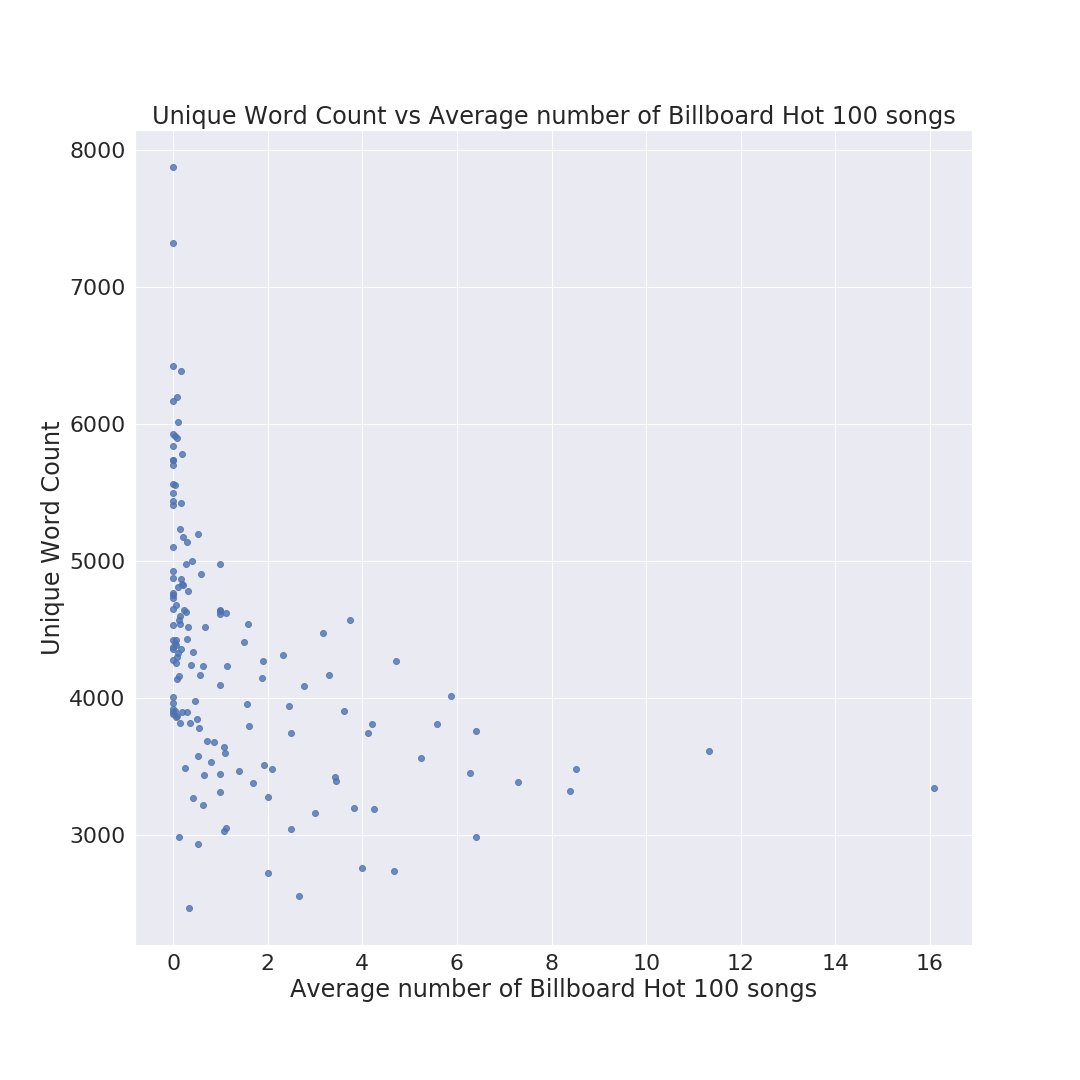
\includegraphics[width=10cm, height=10cm]{./figures/fig1}
	\centering
	\caption{Average number of Billboard 100 songs during artist activity, compared to unique word count across an artists first 35,000 words.}
	\label{fig:fig1}
\end{figure}

\noindent
\newline
To validate the earlier claim that vocabulary range is not indicative of a songwriters ability to write impactful lyrics, the unique word count per artist was compared against the average number of Billboard 100 songs across an artist had across their career. Pearson's Correlation Coefficient , which is used to measure the linear relationship between two variables, was applied to both unique word count and average number of Billboard 100 songs. This resulted in a correlation coefficient of -0.42, indicating a weak inverse correlation between the pairs of data. This value supports the earlier claim that vocabulary range is not indicative of a songwriters ability.

\noindent
\newline
Common methods used to improve songwriting competency include group writing and vocabulary expansion. More recently, software solutions such as MasterWriter(REF) have been used to consolidate previous methods. An inherent problem within software solutions like MasterWriter is the static nature of features such as fixed word and rhyming dictionaries. Consequently, these applications fail to address the ambiguous usage of words resulting from the emerging nature of natural language.

\noindent
\newline
After the completion of song lyrics another secondary problem often faced by less experienced songwriters is choice of instrumental style. 

\section{Goals and Objectives}
\subsection{SONGIFAI - A proposed solution}
The goal of this project is to explore the use of CoVeR derived word embeddings to help with both language modelling and text classification tasks. To contextualise the project aims, both models are applied to a possible use case: a protoype software solution to help reduce common problems faced by songwriters. With this in mind, a prototype solution, SONGIFAI is proposed. SONGIFAI provides two main features namely lyric assistance through predictive text and word suggestions, as well as lyric genre classification. The covariates explored in this project are the following music genres: \textit{Pop}, \textit{Rock} and \textit{Hip-Hop}.
\subsection{High Level Architecture}
\begin{figure}[h]	
	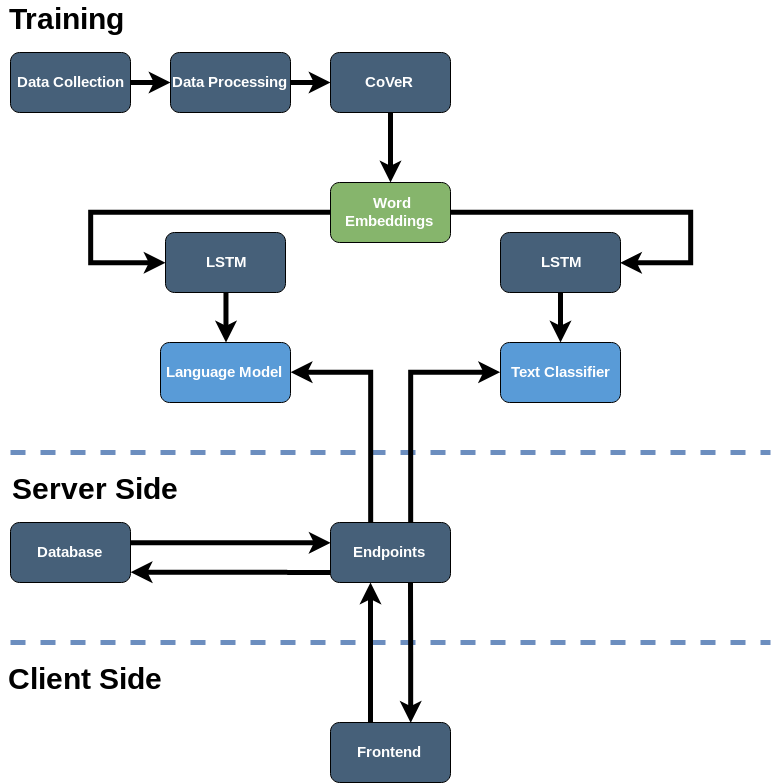
\includegraphics[width=13cm, height=14cm]{./figures/fig7}
	\centering
	\caption{High level architecture for the project}
	\label{fig:fig7}
\end{figure}

 %-----------------------------------------------------
% Chapter: Professional Considerations
%-----
\chapter{Professional Considerations}
\label{prof_con}
Throughout the development of this project professional and ethical considerations will be considered: including those highlighted in the British Computing Societies (BCS) Code of Conduct 4 and Code of Good Practice. The following sections outline relevant areas in the specified documents as well as how this project will adhere to them:
\section{Code of Conduct}
\section{Good Practices}
\section{Ethical Considerations}
The success of this project relies heavily on the availability of correctly labelled lyric data, and as stated before, there is no central repository where lyrics, along with the required metadata for the project, are stored. Consequently, data collection techniques such as web scraping may be used
to gather additional data.
Though web scraping is common practice, it is important to be a “good citizen” of the web and as such the following will be adhered to:
• robots.txt will be obeyed
• requests to sites will be done politely and if stated in the robots.txt file any request rate
limit will be upheld
• the user agent string of the request will be made explicit for the webmaster to see
Due to the nature of the project, appropriate user testing/research will be carried out during development. In accordance with section 1.a of the BCS Code of Conduct, any private data will be stored securely and if possible anonymised.
The project utilises textual data which may have explicit content within it. After the training of models, which will not be filtered to allow artistic freedom into the model, a filtering option will be implemented in order to prevent potential users from seeing explicit content.

%-----------------------------------------------------
% Chapter: Conclusion
%-----------------------------------------------------
\chapter{Conclusion}
\label{chap:conc}

I was right all along.

\section{What was I right about?}

I was right about the following things.

\subsection{Previous theories were wrong}

People thought they understood, but they didn't.

\subsection{My new idea is right}

Of course.


%%%%%%%%%%%%%%%%%%%%%%%%%%%%
% BIBLIOGRAPHY
\clearpage
\phantomsection
\addcontentsline{toc}{chapter}{Bibliography}
\bibliography{bib}
%%%%%%%%%%%%%%%%%%%%%%%%%%%%


%%%%%%%%%%%%%%%%%%%%%%%%%%%%
% START APPENDICES
\appendix
%%%%%%%%%%%%%%%%%%%%%%%%%%%%


%-----------------------------------------------------
% Appendix: Code
%-----------------------------------------------------
\chapter{Code}
\label{app:code}

\begin{verbatim}
10 PRINT "HELLO WORLD"
\end{verbatim}


%%%%%%%%%%%%%%%%%%%%%%%%%%%%
% END DOCUMENT
\end{document}
%%%%%%%%%%%%%%%%%%%%%%%%%%%%